\documentclass[10pt,a4paper]{article}
\usepackage[margin=20mm,top=22mm,bottom=22mm]{geometry}
\usepackage[T1]{fontenc}
\usepackage[utf8]{inputenc}
\usepackage{lmodern}
\usepackage{microtype}
\usepackage{amsmath,amssymb,mathtools}
\usepackage{booktabs,tabularx,array,longtable}
\usepackage{enumitem}
\usepackage{xcolor}
\usepackage{hyperref}
\usepackage{xurl}
\usepackage{fancyhdr}
\usepackage{titlesec}
\usepackage{tcolorbox}
\usepackage{graphicx}
\usepackage{tikz}
\usetikzlibrary{arrows.meta,positioning,calc}
\usepackage{listings}
\usepackage{needspace}
\usepackage{lastpage}
\definecolor{navy}{HTML}{18314D}
\definecolor{blue}{HTML}{245C89}
\definecolor{mint}{HTML}{E7F3EF}
\definecolor{ink}{HTML}{23303D}
\definecolor{slate}{HTML}{536475}
\definecolor{pale}{HTML}{F1F5F9}
\definecolor{line}{HTML}{D8E0E8}
\definecolor{orange}{HTML}{B9682F}
\hypersetup{colorlinks=true,linkcolor=blue,urlcolor=blue,pdftitle={ANDi Research Experiments: Mathematical Methods and Code Changes},pdfauthor={Lab Vision research plan}}
\setlength{\parindent}{0pt}
\setlength{\parskip}{5pt}
\emergencystretch=2em
\setlist[itemize]{leftmargin=16pt,itemsep=2pt,topsep=3pt}
\setlist[enumerate]{leftmargin=18pt,itemsep=3pt,topsep=3pt}
\renewcommand{\arraystretch}{1.18}
\pagestyle{fancy}
\fancyhf{}
\fancyhead[L]{\footnotesize\color{slate} Lab Vision / ANDi research plan}
\fancyhead[R]{\footnotesize\color{slate} 14 November 2026}
\fancyfoot[L]{\footnotesize\color{slate} Experimental proposals - not verified improvements}
\fancyfoot[R]{\footnotesize\color{slate} \thepage/\pageref{LastPage}}
\renewcommand{\headrulewidth}{0.4pt}
\renewcommand{\footrulewidth}{0pt}
\titleformat{\section}{\Large\bfseries\color{navy}}{\thesection}{.7em}{}
\titleformat{\subsection}{\large\bfseries\color{blue}}{\thesubsection}{.6em}{}
\titleformat{\subsubsection}{\normalsize\bfseries\color{navy}}{\thesubsubsection}{.6em}{}
\titlespacing*{\section}{0pt}{16pt}{7pt}
\titlespacing*{\subsection}{0pt}{12pt}{4pt}
\newtcolorbox{summarybox}{colback=pale,colframe=line,boxrule=.65pt,arc=2mm,left=9pt,right=9pt,top=7pt,bottom=7pt}
\newtcolorbox{attentionbox}{colback=white,colframe=orange,boxrule=.8pt,arc=1.5mm,left=9pt,right=9pt,top=6pt,bottom=6pt}
\newcommand{\file}[1]{\nolinkurl{#1}}
\newcommand{\hyps}[1]{\begin{summarybox}\textbf{Research question.} #1\end{summarybox}}
\newcommand{\flowsteps}[4]{%
\begin{center}\begin{tikzpicture}[node distance=1.6mm, every node/.style={font=\footnotesize}, >=Latex]
\node[draw=line,rounded corners=2pt,fill=pale,minimum width=.87\linewidth,text width=.82\linewidth,align=center,inner ysep=5pt] (a) {#1};
\node[draw=line,rounded corners=2pt,fill=pale,below=of a,minimum width=.87\linewidth,text width=.82\linewidth,align=center,inner ysep=5pt] (b) {#2};
\node[draw=line,rounded corners=2pt,fill=pale,below=of b,minimum width=.87\linewidth,text width=.82\linewidth,align=center,inner ysep=5pt] (c) {#3};
\node[draw=blue,rounded corners=2pt,fill=mint,below=of c,minimum width=.87\linewidth,text width=.82\linewidth,align=center,inner ysep=5pt] (d) {#4};
\draw[->,color=slate] (a)--(b);\draw[->,color=slate] (b)--(c);\draw[->,color=slate] (c)--(d);
\end{tikzpicture}\end{center}}
\lstdefinestyle{andi}{language=Python,basicstyle=\ttfamily\scriptsize,keywordstyle=\color{blue}\bfseries,commentstyle=\color{slate},stringstyle=\color{orange},backgroundcolor=\color{pale},frame=single,rulecolor=\color{line},framerule=.5pt,breaklines=true,showstringspaces=false,xleftmargin=6pt,xrightmargin=6pt,aboveskip=5pt,belowskip=5pt}
\lstset{style=andi}
\begin{document}
\begin{flushleft}
{\color{blue}\textbf{UNIVERSITY OF BONN \; / \; LAB VISION}}\\[9pt]
{\Huge\bfseries\color{navy} ANDi Research Experiments}\\[7pt]
{\Large\color{slate} Mathematics, procedures and code modifications}\\[11pt]
{\small\color{slate} Research planning document \quad | \quad 14 November 2026}
\end{flushleft}
\vspace{4mm}
\begin{summarybox}
\textbf{Scope.} This document describes five proposed experiments discussed after the ANDi supervision meeting: three \textbf{inference-only} methods and two \textbf{training-based} extensions. All are research ideas to investigate as time permits, not guaranteed improvements. Synthetic-\emph{anomaly training} is intentionally excluded; synthetic lesions are used only for threshold calibration in Experiment 2.\par
\textbf{Recommended order.} Verify baseline $\rightarrow$ inference-only experiments $\rightarrow$ training extensions if time and compute allow. Each experiment should be interpretable as a standalone ablation.
\end{summarybox}
\vspace{2mm}
\begin{center}
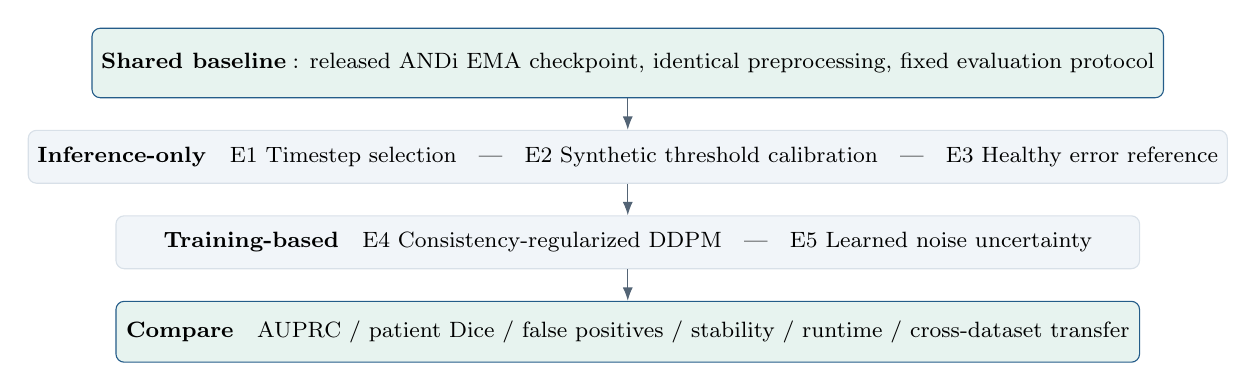
\begin{tikzpicture}[>=Latex,font=\footnotesize,node distance=4mm]
\node[draw=blue,fill=mint,rounded corners=3pt,minimum width=13cm,inner ysep=9pt,align=center] (a) {\textbf{Shared baseline}\;: released ANDi EMA checkpoint, identical preprocessing, fixed evaluation protocol};
\node[draw=line,fill=pale,rounded corners=3pt,below=of a,minimum width=13cm,inner ysep=6pt,align=center] (b) {\textbf{Inference-only}\quad E1 Timestep selection \; | \; E2 Synthetic threshold calibration \; | \; E3 Healthy error reference};
\node[draw=line,fill=pale,rounded corners=3pt,below=of b,minimum width=13cm,inner ysep=6pt,align=center] (c) {\textbf{Training-based}\quad E4 Consistency-regularized DDPM \; | \; E5 Learned noise uncertainty};
\node[draw=blue,fill=mint,rounded corners=3pt,below=of c,minimum width=13cm,inner ysep=7pt,align=center] (d) {\textbf{Compare}\quad AUPRC / patient Dice / false positives / stability / runtime / cross-dataset transfer};
\draw[->,color=slate] (a)--(b);\draw[->,color=slate] (b)--(c);\draw[->,color=slate] (c)--(d);
\end{tikzpicture}
\end{center}
\vspace{2mm}
\textbf{Notation.} $x_0$: MRI slice; $x_t$: corrupted slice; $t$: diffusion index; $c$: MRI modality; $p$: voxel/pixel; $d_{t,c}(p)$: ANDi squared reverse-transition discrepancy; $A(p)$: aggregate anomaly score; $M$: binary lesion mask; $\theta$: denoiser parameters.
\newpage
\section{Common baseline, data controls and success criteria}
\subsection{Mathematical reference}
For an observed MRI slice $x_0$ and timestep $t$, the released model samples standard Gaussian evaluation noise $\epsilon$ and computes
\begin{align}
 x_t &=\sqrt{\bar\alpha_t}\,x_0 + \sqrt{1-\bar\alpha_t}\,\epsilon,\\
 \widehat\epsilon &=\epsilon_\theta(x_t,t),\\
 d_{t,c}(p)&=\left[\frac{\beta_t}{\sqrt{\alpha_t}\sqrt{1-\bar\alpha_t}}\right]^2
 (\epsilon_c(p)-\widehat\epsilon_c(p))^2.
\end{align}
The original method uses $\mathcal T_0=\{75,\ldots,199\}$, $K=125$, and
\begin{equation}
 A_c(p)=\exp\!\left(\frac{1}{K}\sum_{t\in\mathcal T_0}\log(d_{t,c}(p)+\delta)\right),\qquad
 A(p)=\max_{c=1,\ldots,4}A_c(p).
\end{equation}
Here $\delta>0$ is a numerical-stability addition for new implementations; the released \file{utils.py} \file{gmean()} does \emph{not} add it. To exactly reproduce the released pipeline, preserve the old behavior separately and only use stabilized aggregation in controlled ablations.

\subsection{Protocol frozen for all experiments}
\begin{enumerate}
\item \textbf{Inputs:} same four MRI modalities, registration/histogram-matching choices, 99th-percentile normalization and spatial resizing as the original baseline.
\item \textbf{Splits:} fixed BraTS21 train/validation/test lists. Reserve test labels and test scores for final assessment, not method selection. MSSEG and Ljubljana are independent transfer tests where available.
\item \textbf{Reference model:} released EMA checkpoint; fixed seed(s). Reproduce unfiltered, 3$\times$3$\times$3 and 5$\times$5$\times$5 median-filter results before comparisons.
\item \textbf{Evaluation:} pooled voxel average precision (AUPRC/AP), mean patient-level Dice, optionally FPR at fixed recall, paired subject-level confidence intervals, and wall-clock inference time including the same preprocessing scope.
\item \textbf{Comparability:} freeze the postprocessing, brain mask, threshold calibration rule, and any score scaling when isolating a specific change. Treat nonlesion voxels of tumor-bearing subjects differently from a genuinely healthy cohort.
\end{enumerate}
\begin{attentionbox}
\textbf{Key evaluation caution.} AUPRC measures \emph{ranking}; changing only a binary threshold cannot increase AUPRC. A positive global rescaling likewise leaves AUPRC unchanged. The existing \file{eval.py} performs dataset-wide min--max score normalization; for transferable calibrated thresholds use a predefined and consistently applied score scale, not a new scale inferred from the held-out test cohort.
\end{attentionbox}
\subsection{Baseline code entry points}
\begin{tabularx}{\linewidth}{@{}p{37mm}X@{}}
\toprule
File & Role to preserve / extend\\\midrule
\file{diffusion.py} & \file{Diffusion.normative_diffusion()} samples $t$, evaluates U-Net and returns all $d_t$ maps.\\
\file{eval.py} & Converts volumes to slices, calls diffusion, aggregates timesteps/channels, median-filters, normalizes, thresholds and scores.\\
\file{utils.py} & \file{gmean()}, \file{median_filter_3D()}, \file{norm_tensor()}, \file{dice()}.\\
\file{train.py} & Loads healthy-slice LMDB, draws timestep and pyramidal noise, computes MSE, updates model/EMA.\\
\file{modules.py} & Time-conditioned U-Net, presently 4-channel noise output.\\
\file{conf/eval.yml} / \file{conf/train.yml} & Central experiment settings and reproducibility controls.\\\bottomrule
\end{tabularx}
\newpage
\section{E1. Timestep subset selection (inference-only)}
\hyps{Can a smaller, carefully chosen subset of diffusion timesteps preserve or improve ANDi segmentation accuracy while reducing inference cost?}
\subsection{Motivation and mathematics}
The baseline evaluates every timestep $t\in\mathcal T_0$, yet some error maps may be redundant. Choose $S\subseteq\mathcal T_0$ with $|S|=k$ and compute
\begin{equation}
 A_{c,S}(p)=\exp\left[\frac1k\sum_{t\in S}\log(d_{t,c}(p)+\delta)\right],\qquad
 A_S(p)=\max_c A_{c,S}(p).
\end{equation}
Investigate \emph{uniformly spaced}, \emph{random}, \emph{contiguous low/high-noise windows} and \emph{correlation-aware} selections, for $k\in\{10,25,50,75,125\}$. If $R_{ij}$ is the correlation of flattened log-residual maps at timesteps $i,j$ on calibration subjects, one label-free diversity criterion is
\begin{equation}
 S^*=\arg\min_{S\subseteq\mathcal T_0,\,|S|=k}\frac{2}{k(k-1)}\sum_{i<j,\,i,j\in S}|R_{ij}|.
\end{equation}
Purely minimizing redundancy may select uninformative timesteps; also report each timestep's error distribution and investigate a simple predeclared window/stratification rule. Any criterion optimized using real lesion AP/Dice is \emph{supervised validation}, not label-free selection.
\subsection{Use the noise schedule as a sampling coordinate}
The original ANDi window is $\mathcal T_0=\{75,\ldots,199\}$ (125 steps; \file{conf/eval.yml}: \texttt{stop: 200} is exclusive), \emph{not} $125$--$199$. A window beginning at $125$ is a candidate for ablation. The original DDPM configuration fixes
\begin{equation}
 \beta_t=10^{-4} + (0.02-10^{-4})\frac{t}{999},\quad
 \alpha_t=1-\beta_t,\quad
 \bar\alpha_t=\prod_{j=0}^{t}\alpha_j.
\end{equation}
For the exact zero-based arrays in \file{diffusion.py}, define the squared coefficients of the original signal and Gaussian corruption as
\begin{equation}
 Q_{\rm signal}(t)=\bar\alpha_t,\qquad Q_{\rm noise}(t)=1-\bar\alpha_t.
\end{equation}
The values below come from the actual linear schedule in \file{conf/eval.yml} (1000 elements). They quantify the mixing \emph{coefficients}, not the percentage of recognizable MRI anatomy or necessarily the fraction of empirical image variance.
\begin{center}
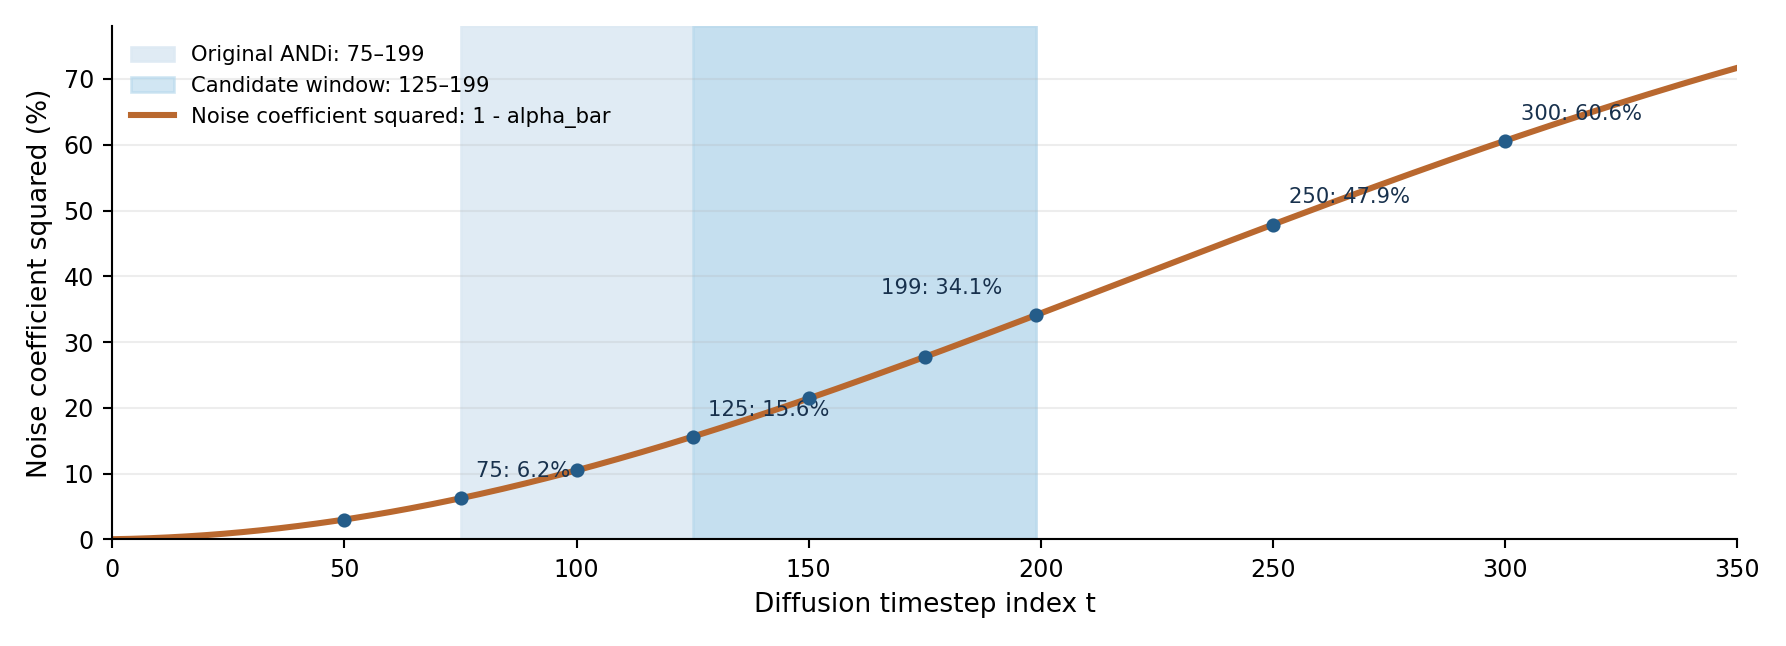
\includegraphics[width=.92\linewidth]{noise_schedule.png}
\end{center}
\begin{center}
\small
\begin{tabular}{@{}lrrrrr@{}}
\toprule
$t$ & 50 & 75 & 100 & 125 & 150 \\\midrule
$100Q_{\rm noise}(t)$ & 3.0 & 6.2 & 10.5 & 15.6 & 21.4 \\
\midrule
$t$ & 175 & 199 & 250 & 300 & -- \\\midrule
$100Q_{\rm noise}(t)$ & 27.7 & 34.1 & 47.9 & 60.6 & -- \\\bottomrule
\end{tabular}
\end{center}
Within 75--199 the squared noise coefficient grows from about $6.2\%$ to $34.1\%$. Hence equal differences in $t$ do \emph{not} correspond to equal differences in corruption strength. We can use this known schedule to design nonuniform subsets \emph{before} measuring any lesion labels.
\subsection{Additional selection policies}
For a candidate range $[t_{\min},t_{\max}]$ and a budget $k$, compare the following strategies under the \emph{same} checkpoint, postprocessing and inference evaluation:
\par\medskip\noindent\begin{tabularx}{\linewidth}{@{}p{34mm}X@{}}
\toprule Policy & Selection rule and question tested\\\midrule
Uniform timestep & Select $k$ equally spaced integer indices in the window: is naive thinning sufficient?\\
Uniform noise fraction & Sample $k$ equally spaced targets between $Q_{\rm noise}(t_{\min})$ and $Q_{\rm noise}(t_{\max})$; map each to its nearest unused integer timestep. Does explicit corruption-level coverage help?\\
Uniform log-SNR & With $\ell_t=\log[\bar\alpha_t/(1-\bar\alpha_t)]$, space targets evenly in $\ell_t$ and find nearest unused steps. Does relative SNR coverage help?\\
Random subset & Sample $k$ unique timesteps without replacement; repeat across selection seeds to establish a variability baseline.\\
Correlation-aware & Estimate residual-map correlations from independent calibration subjects and choose less-redundant timesteps. Use no test labels for subset construction.\\\bottomrule
\end{tabularx}\par\medskip
In mathematical form, the two schedule-aware policies solve the same nearest-step assignment problem. Define $g(t)$ as either $Q_{\rm noise}(t)$ or $\ell_t$, let
\begin{equation}
 u_i=g(t_{\min})+\frac{i}{k-1}\big[g(t_{\max})-g(t_{\min})\big],\quad i=0,\ldots,k-1,
\end{equation}
and select an unused $t_i\in[t_{\min},t_{\max}]$ minimizing $|g(t_i)-u_i|$. Enforce $k$ \emph{distinct} indices; rounding/nearest-neighbor matching can otherwise duplicate timesteps.
\subsection{Separate efficiency from noise-window sensitivity}
Test two independent axes rather than changing the window and step count together:
\begin{enumerate}
\item \textbf{Fixed window, changing budget:} hold 75--199 and compare $k\in\{10,25,50,75,125\}$ for uniform-$t$, uniform-noise, uniform-log-SNR, random, and correlation-aware selection. This isolates sparsification and tests the performance--runtime tradeoff.
\item \textbf{Fixed budget, changing window:} hold e.g. $k=25$ and explore 50--124, 75--149, 75--199, 125--199, 100--224, and 50--249. The windows outside the paper's 75--199 setting are \emph{exploratory} and may involve different learned noise regimes; tune using calibration/validation subjects only.
\end{enumerate}
Quantify actual measured speed-up, not only the ideal reduction in neural evaluations:
\begin{equation}
 \operatorname{Speedup}(S)=\frac{\operatorname{median}\,\mathrm{runtime}(\mathcal T_0)}{\operatorname{median}\,\mathrm{runtime}(S)},\qquad
 \operatorname{IdealReduction}=1-\frac{k}{125}.
\end{equation}
Use synchronized GPU timing and consistent batch sizes. The final report should contain paired AUPRC/Dice change against baseline \emph{versus} wall-clock latency and speed-up, with variability across subjects and random selections. Plot both ranking quality (AP) and segmentation quality (Dice); also show a timestep-level AP diagnostic on validation data, explicitly marking it as label-dependent descriptive analysis, \emph{not} a label-free selection score.

\subsection{Procedure}
\flowsteps{Run the frozen checkpoint once over all 125 timesteps on calibration subjects; save log-residual maps or summarized per-timestep features.}{Analyze residual histograms, pairwise correlations and spatial stability across timesteps.}{Construct subsets at each budget $k$: uniform, repeated random draws, low/high windows and diversity-based.}{Apply only selected steps at actual inference; plot AUPRC and Dice against measured latency / speed-up.}
\begin{enumerate}
\item Use the same noise draw for each $(\text{subject},t)$ across competing selection methods; seed repeated trials separately.
\item Apply exactly the same modality max, 3D filtering and threshold rule to each selected subset.
\item For random subsets, report variability across several independent subset draws; separately study noise-seed variability.
\item Verify real speed by executing the reduced number of U-Net evaluations, not simply estimating time from stored maps.
\end{enumerate}
\subsection{What to change in code}
\begin{tabularx}{\linewidth}{@{}p{37mm}X@{}}
\toprule File & Modification\\\midrule
\file{diffusion.py} & Add optional \file{timesteps} parameter to \file{normative_diffusion()}; validate unique indices; iterate over selected indices; allocate $k$ maps rather than \file{stop-start}; write to subset index instead of \file{i-start}. Keep original default path intact.\\
\file{eval.py} & Pass selected indices from config; optionally cache time-indexed residuals before geometric aggregation; log GPU time and end-to-end time.\\
\file{conf/eval.yml} & Add \file{selection_method}, \file{sampling_space: timestep|noise|log_snr}, \file{num_timesteps}, \file{window_start}, \file{window_end} (inclusive), \file{timesteps}, and \file{seed}.\\
New \file{experiments/select_timesteps.py} & Compute subset indices and redundancy matrices using calibration data only; save reproducible subsets as JSON.\\\bottomrule
\end{tabularx}
\begin{lstlisting}
# Schematic replacement for the timestep loop in diffusion.py
steps = list(range(start, stop)) if timesteps is None else sorted(set(timesteps))
dts = torch.empty((num_images, len(steps), *images.shape[1:]), device=self.device)
for j, step in enumerate(steps):
    t = torch.full((num_images,), step, dtype=torch.long, device=self.device)
    x_t, eps = self.noise_images(images, t, pyramid=pyramid, discount=discount)
    pred = model(x_t, t)
    dts[:, j] = (self.ddpm_mu_t(x_t, eps, t) -
                 self.ddpm_mu_t(x_t, pred, t)).square()
\end{lstlisting}
\begin{lstlisting}
# Additional selection logic for experiments/select_timesteps.py
# alpha_hat: 1000-element cumulative-product tensor from Diffusion
alpha = alpha_hat.detach().cpu().numpy()
noise_fraction = 1.0 - alpha
log_snr = np.log(alpha / (1.0 - alpha))

def schedule_subset(start, end, k, space="noise"):
    # `end` is inclusive here; normative_diffusion receives the list.
    indices = list(range(start, end + 1))
    assert 2 <= k <= len(indices)
    signal = noise_fraction if space == "noise" else log_snr
    targets = np.linspace(signal[start], signal[end], k)
    available = set(indices)
    chosen = []
    for target in targets:
        t = min(available, key=lambda i: abs(signal[i] - target))
        available.remove(t)
        chosen.append(t)
    return sorted(chosen)

steps = schedule_subset(75, 199, 25, space="noise")
# Compare against 25 uniformly spaced t indices and repeated random subsets.
\end{lstlisting}
\textbf{Interpretation caution.} The previous interactive graphic only shows $Q_{\rm noise}(t)$, a property of the \emph{fixed beta schedule}. It cannot establish which timesteps actually improve lesion detection. That requires per-timestep residuals, controlled comparisons and an independently evaluated accuracy--latency curve.\par
\textbf{Deliverables:} timestep correlation heatmap; performance--latency Pareto plot; representative lesion maps; table of $k$ versus mean and variance of Dice/AP, GPU memory and latency.\par
\textbf{Main risk:} lower $k$ reduces stochastic averaging; an apparent speed improvement can come at the cost of unstable small-lesion detection.
\Needspace{12\baselineskip}
\section{E2. Synthetic-lesion threshold calibration (inference-only)}
\hyps{Can synthetic lesions determine a useful ANDi segmentation threshold without using real lesion masks for threshold selection?}
\subsection{Motivation and mathematics}
The frozen ANDi scores can rank lesions well yet Yen thresholding may be suboptimal. Construct pseudo-anomalous images from truly healthy (preferred) or explicitly nonlesion training/validation slices. With synthetic lesion mask $M_{\rm syn}(p)\in\{0,1\}$ and lesion operator $G$, use
\begin{equation}
 x_{\rm syn}(p)=(1-M_{\rm syn}(p))x_H(p)+M_{\rm syn}(p)G(x_H,p).
\end{equation}
The operator should preserve normal image values outside the mask and create multi-modal, spatially coherent intensity changes within it. Obtain the frozen-model anomaly map $A(x_{\rm syn})$, then fit a fixed threshold or subject-adaptive threshold parameter, for example
\begin{align}
 \tau^*&=\arg\max_{\tau}\frac1N\sum_{j=1}^N
 \mathrm{Dice}\big(\mathbf1[A_j>\tau],M_{{\rm syn},j}\big),\\
 \tau_j(k)&=\mathrm{median}_{p\in B_j}A_j(p)
 +k\,\mathrm{MAD}_{p\in B_j}A_j(p).
\end{align}
A $k$ value may likewise be selected by synthetic-mask Dice. Optimize either $\tau$ or $k$ on \emph{synthetic calibration data only}, then freeze it before real test evaluation. This uses synthetic-mask supervision, not real-lesion-label supervision.
\subsection{Procedure}
\flowsteps{Sample clean axial MR slices and brain-valid candidate lesion locations.}{Generate irregular connected lesion masks; insert mild/strong lesions at several sizes and across MRI modalities.}{Run the released, frozen ANDi scoring; choose $\tau$ or $k$ on synthetic masks with frozen postprocessing.}{Evaluate real BraTS21 test and Shifts cases; compare Dice to Yen at unchanged AUPRC.}
\begin{enumerate}
\item Make lesion size and texture distributions explicit; compare small MS-like and large tumor-like families without tailoring them from test labels.
\item Split synthetic source subjects into calibration and model-selection groups to prevent overfitting to the generator.
\item Include healthy-only controls to quantify false positives; test at least two distinct synthetic generators to probe shortcut learning.
\item Evaluate with and without the \emph{same} dilation as the Yen baseline. Maintain the original score units or a calibration-defined transformation.
\end{enumerate}
\subsection{What to change in code}
\begin{tabularx}{\linewidth}{@{}p{39mm}X@{}}
\toprule File & Modification\\\midrule
New \file{experiments/synthetic_lesions.py} & Load clean 4-channel slices and construct $M_{\rm syn}$ plus paired $x_{\rm syn}$. Keep images and masks aligned; save lesion-generator settings and seeds.\\
New \file{experiments/threshold_calibration.py} & Cache synthetic anomaly maps, sweep $\tau$ or $k$, select on synthetic masks, save thresholds and validation metadata.\\
\file{eval.py} & Add \file{threshold_method: yen|fixed|subject_mad}, apply per-subject thresholds, and evaluate separate postprocessing variants.\\
\file{conf/eval.yml} & Add threshold config and path to frozen threshold JSON; do not fit threshold during test evaluation.\\\bottomrule
\end{tabularx}
\begin{lstlisting}
# Scoring and threshold selection are separate stages
A_syn = compute_andi_scores(x_syn, frozen_checkpoint)
for tau in candidate_thresholds:
    dice_by_subject[tau] = mean_subject_dice(A_syn > tau, synthetic_masks)
tau_star = max(dice_by_subject, key=dice_by_subject.get)
save_json({'tau': tau_star, 'generator_seed': seed})
# Later: apply tau_star to untouched real-test anomaly maps
\end{lstlisting}
\textbf{Deliverables:} selected threshold, calibration curve, synthetic-vs-real robustness table, Dice/FPR and lesion-size stratification.\par
\textbf{Main risk:} easy-to-spot synthetic boundaries can tune a threshold that fails on subtle real lesions. This experiment changes thresholding, not the underlying AUPRC ranking.
\Needspace{12\baselineskip}
\section{E3. Healthy-reference residual calibration (inference-only)}
\hyps{Can the healthy distribution of per-timestep denoising errors identify unusually large residuals better than raw ANDi aggregation?}
\subsection{Motivation and mathematics}
Alex's notes propose estimating healthy residual statistics by timestep and MRI modality, then standardizing before aggregation. Let $d_{t,c}^{(j)}(p)$ be the error on healthy-reference subject $j$. Use $\ell_{t,c}=\log(d_{t,c}+\delta)$ and estimate
\begin{equation}
 \mu_{t,c}=\mathbb E_{(j,p)\in H}[\ell_{t,c}^{(j)}(p)],\qquad
 \sigma_{t,c}^2=\mathrm{Var}_{(j,p)\in H}[\ell_{t,c}^{(j)}(p)].
\end{equation}
Then compute standardized log-error
\begin{equation}
 z_{t,c}(p)=\frac{\log(d_{t,c}(p)+\delta)-\mu_{t,c}}
 {\max(\sigma_{t,c},\sigma_{\min})}.
\end{equation}
A signed $z$ value cannot directly enter the old geometric-mean function (which takes a logarithm of nonnegative scores). Use a \emph{defined, valid} aggregate, such as
\begin{equation}
 A^{\rm ref}_c(p)=\frac{1}{K}\sum_{t\in\mathcal T_0}\max\{0,z_{t,c}(p)\},
 \qquad A^{\rm ref}(p)=\max_c A^{\rm ref}_c(p).
\end{equation}
A secondary ablation may use $\mathrm{softplus}(z)$ instead of clipping. Because $\sigma_{t,c}$ depends on time and modality, dividing by it reweights the terms; it is not merely one global rescaling. Avoid choosing $\mu,\sigma$ from held-out test subjects.
\subsection{Procedure}
\flowsteps{Run the frozen model on an independent healthy-reference cohort (or clearly labelled nonlesion calibration voxels).}{For each $t,c$, estimate robust statistics of log-residual scores; store reference parameters and counts.}{At test time, standardize each $d_{t,c}$, aggregate valid nonnegative anomaly evidence, and apply unchanged spatial processing.}{Compare uncalibrated vs calibrated AUPRC, Dice, healthy FPR and transfer to MS cohorts.}
\begin{enumerate}
\item Compare scalar per-$(t,c)$ reference statistics with an optional region/tissue-conditioned extension only if the initial method warrants it.
\item Study mean/std versus median/MAD, and report distribution plots before and after calibration.
\item Check whether high normal variance overlaps with lesion-prone anatomy; compare separately to existing negative exploratory atlas-score results.
\item Keep threshold selection comparable. Score normalization changes ranking; AUPRC is the primary diagnostic.
\end{enumerate}
\subsection{What to change in code}
\begin{tabularx}{\linewidth}{@{}p{39mm}X@{}}
\toprule File & Modification\\\midrule
\file{diffusion.py} & Keep or expose the full $d_{t,c}$ tensor before aggregate; optionally stream sufficient statistics to reduce memory.\\
New \file{experiments/fit_healthy_stats.py} & Compute $\mu_{t,c}$, $\sigma_{t,c}$ and reference sample counts on calibration subjects. Save checkpoint/config ID.\\
\file{eval.py} & Add \file{aggregation_method: original|healthy_z} and apply standardization on time-indexed maps before max-over-modalities.\\
\file{utils.py} & Add stable \file{aggregate_standardized_residuals()}\; do not pass signed z-scores into \file{gmean()}.\\\bottomrule
\end{tabularx}
\begin{lstlisting}
# dts shape: [slices, time, modality, height, width]
log_d = torch.log(dts.clamp_min(delta))
z = (log_d - mu_tc[None, :, :, None, None]) / \
    sigma_tc.clamp_min(sigma_floor)[None, :, :, None, None]
A_modality = torch.relu(z).mean(dim=1)  # explicit positive-evidence rule
A_slice = A_modality.amax(dim=1)
\end{lstlisting}
\textbf{Deliverables:} reference distributions, per-timestep/modality z-score histograms, AUPRC and Dice ablations, examples of false-positive changes.\par
\textbf{Main risk:} nonlesion voxels in tumor-bearing scans are imperfect healthy references. Standardization can suppress true lesions in intrinsically high-variance regions, as suggested by earlier exploratory results.
\Needspace{12\baselineskip}
\section{E4. Consistency-regularized diffusion training (training-based)}
\hyps{Can encouraging consistent denoising predictions under harmless MRI intensity transformations improve robustness to nonpathological scanner and contrast variability?}
\subsection{Motivation and mathematics}
This interprets Alex's handwritten \emph{additional loss} as a consistency penalty; it is not ordinary L2 weight decay. For a healthy slice $x_0$, generate a small, approximately pathology-preserving intensity transform $g(x_0)$ (gamma, smooth bias field, or modest contrast scaling). Apply the \emph{same} timestep $t$ and the \emph{same} pyramidal noise $\epsilon$ to both:
\begin{align}
 x_t&=\sqrt{\bar\alpha_t}x_0+\sqrt{1-\bar\alpha_t}\epsilon,\\
 \widetilde x_t&=\sqrt{\bar\alpha_t}g(x_0)+\sqrt{1-\bar\alpha_t}\epsilon.
\end{align}
The proposed consistency regularizer is
\begin{equation}
 \mathcal L_{\rm cons}=\mathbb E\left[\left\|\epsilon_\theta(x_t,t)-
 \epsilon_\theta(\widetilde x_t,t)\right\|_2^2\right].
\end{equation}
A sensible total objective also trains both branches to predict the same known noise:
\begin{align}
 \mathcal L_{\rm DDPM}^{\rm pair}&=\frac12\mathbb E\Big[
 \|\epsilon-\epsilon_\theta(x_t,t)\|_2^2+
 \|\epsilon-\epsilon_\theta(\widetilde x_t,t)\|_2^2\Big],\\
 \mathcal L_{\rm total}&=\mathcal L_{\rm DDPM}^{\rm pair}+\lambda_{\rm cons}\mathcal L_{\rm cons}.
\end{align}
Training branches with identical noise gives the consistency target a clear interpretation: the predicted corruption should be insensitive to the chosen harmless change in healthy tissue appearance. This is a \emph{hypothesis}, and overly strong invariance may erase useful lesion-related sensitivity.
\subsection{Procedure}
\flowsteps{Take an unmodified healthy training slice and a mild appearance-transformed version $g(x_0)$.}{Noise both using identical sampled timestep and pyramid noise; predict $\epsilon$ with a shared U-Net.}{Optimize paired DDPM MSE plus $\lambda_{\rm cons}$ times prediction consistency; maintain EMA checkpoint.}{Run unchanged ANDi evaluation and test robustness on BraTS21, Ljubljana and MSSEG.}
\begin{enumerate}
\item Start with a no-consistency \emph{augmentation-only} control and $\lambda=0$ baseline; then a small, predeclared $\lambda$ grid. Avoid selecting based on test labels.
\item Ensure $g$ preserves background mask and anatomy. Use restrained, physically plausible intensity changes rather than geometric displacements.
\item Compare original checkpoint, augmentation-only model, and augmentation-plus-consistency model under identical inference settings.
\item Measure training overhead: the second forward pass raises compute substantially; training time must be benchmarked on Bender.
\end{enumerate}
\subsection{What to change in code}
\begin{tabularx}{\linewidth}{@{}p{39mm}X@{}}
\toprule File & Modification\\\midrule
\file{train.py} & After sampling healthy image, $t$ and pyramid noise, create $g(x_0)$; form two $x_t$ tensors with the same $\epsilon$; compute paired MSE and consistency MSE; log both.\\
\file{utils.py} or new \file{augmentations.py} & Add differentiable/intensity-only transformation functions with controlled ranges and reproducible seeds.\\
\file{conf/train.yml} & Add \file{consistency_lambda}, \file{augmentation_type}, magnitude and seed settings; keep a baseline-compatible default of zero.\\
\file{modules.py} & No architectural change required; use existing U-Net shared across both training branches.\\\bottomrule
\end{tabularx}
\begin{lstlisting}
# Sketch inside train.py (pyramidal eps reused for both images)
x_aug = healthy_intensity_augment(images)
t = diffusion.sample_timesteps(images.shape[0]).to(device)
x_t, eps = diffusion.noise_images(images, t, pyramid=True)
a = diffusion.alpha_hat[t][:, None, None, None]
x_t_aug = a.sqrt() * x_aug + (1 - a).sqrt() * eps
pred, pred_aug = model(x_t, t), model(x_t_aug, t)
L_ddpm = 0.5 * (mse(pred, eps) + mse(pred_aug, eps))
L_cons = mse(pred, pred_aug)
loss = L_ddpm + lambda_cons * L_cons
\end{lstlisting}
\textbf{Deliverables:} loss-component curves, hyperparameter ablation, robustness under synthetic scanner shifts, external-test AUPRC/Dice.\par
\textbf{Main risk:} augmentations that are too strong or unrealistic can degrade the learned normative distribution; consistency may encourage the model to ignore meaningful changes.
\Needspace{12\baselineskip}
\section{E5. Predictive-noise uncertainty learning (training-based)}
\hyps{Can a denoiser that learns the variability of healthy noise-prediction errors produce better-calibrated anomaly scores than unweighted squared errors?}
\subsection{Motivation and mathematics}
The current U-Net emits four noise channels, $\widehat\epsilon=\epsilon_\theta(x_t,t)$, and training minimizes MSE. A proposed extension predicts both a conditional mean $m_\theta$ and per-coordinate log-variance $s_\theta=\log\sigma_\theta^2$ of the \emph{noise prediction target}:
\begin{equation}
 p_\theta(\epsilon\mid x_t,t)=\mathcal N\!\left(m_\theta(x_t,t),
 \operatorname{diag}(e^{s_\theta(x_t,t)})\right).
\end{equation}
The heteroscedastic Gaussian negative log-likelihood, ignoring its constant, is
\begin{equation}
 \mathcal L_{\rm NLL}=
 \frac12\,\mathbb E\left[\sum_p
 e^{-s_\theta(p)}(\epsilon(p)-m_\theta(p))^2+s_\theta(p)
 \right].
\end{equation}
At inference, two candidate anomaly scores are (i) the standardized squared residual $r_t=(\epsilon-m_\theta)^2/(e^{s_\theta}+\delta)$, and (ii) the full NLL contribution $\frac12[r_t+s_\theta]$. The first is nonnegative and can enter a geometric mean; the second may be negative, so aggregate it in log-score space by an arithmetic mean, not by taking its logarithm:
\begin{align}
 A_c^{\rm std}(p)&=\exp\left[\frac1K\sum_t\log(r_{t,c}(p)+\delta)\right],\\
 A_c^{\rm NLL}(p)&=\frac1{2K}\sum_t[r_{t,c}(p)+s_{t,c}(p)].
\end{align}
\textbf{Scientific distinction:} this models heteroscedastic uncertainty for the predicted \emph{noise target}; it is not identical to learning the DDPM reverse-transition variance $\Sigma_\theta(x_t,t)$ in Improved DDPM. Both are possible but different experiments.
\subsection{Procedure}
\flowsteps{Modify U-Net final output from four to eight channels, split into predicted noise mean and log-variance.}{Train on healthy slices with Gaussian NLL; constrain/clamp log-variance and monitor calibration.}{At test time, calculate standardized squared residual and NLL scores across timesteps.}{Compare with original MSE-based ANDi and evaluate whether uncertainty removes false positives or suppresses lesions.}
\begin{enumerate}
\item Compare MSE-only, mean+variance NLL, and a hybrid loss; monitor variance collapse or inflation.
\item Calibrate variance on held-out healthy data. Check residual calibration before evaluating pathology.
\item Control architecture/output-head size and training budget; do not attribute improvement solely to uncertainty if training schedule changes.
\item Test external scanner transfer, particularly where healthy uncertainty estimates may be poorly calibrated.
\end{enumerate}
\subsection{What to change in code}
\begin{tabularx}{\linewidth}{@{}p{39mm}X@{}}
\toprule File & Modification\\\midrule
\file{modules.py} & Change \file{UNet(c_out=8)} or implement two 4-channel heads. Split into noise mean and log-variance. The 4-channel EMA checkpoint is not directly loadable into an 8-channel final layer; initialize/transfer weights deliberately.\\
\file{train.py} & Replace or augment \file{nn.MSELoss()} with heteroscedastic Gaussian NLL; log mean residual, log-variance range, and calibration statistics.\\
\file{diffusion.py} & Add a separate uncertainty-scoring function returning per-time NLL or standardized residual maps; preserve the original \file{normative_diffusion()} path.\\
\file{eval.py} & Add \file{score_type: original|standardized|nll} with mathematically compatible aggregation rules.\\
\file{conf/train.yml} & Add variance clamp range, loss type, and any hybrid MSE weight.\\\bottomrule
\end{tabularx}
\begin{lstlisting}
# Sketch: model returns 8 channels; 4 mean and 4 log-variance
out = model(x_t, t)
mean_eps, log_var = out.chunk(2, dim=1)
log_var = log_var.clamp(min=-8.0, max=4.0)  # illustrative bounds
sq_error = (noise - mean_eps).square()
loss_nll = 0.5 * (sq_error * torch.exp(-log_var) + log_var).mean()
# Inference: standardized error is nonnegative
score_t = sq_error / (torch.exp(log_var) + 1e-8)
\end{lstlisting}
\textbf{Deliverables:} predicted variance maps, healthy residual calibration plots, NLL-vs-MSE anomaly map comparisons, and performance/compute ablations.\par
\textbf{Main risk:} high predicted variance in a lesion region can suppress its standardized anomaly signal; model variance on out-of-distribution cases is not guaranteed to be trustworthy.
\Needspace{12\baselineskip}
\section{Experiment ordering, code inventory and decision criteria}
\subsection{Proposed execution sequence}
\begin{tabularx}{\linewidth}{@{}p{13mm}p{48mm}X@{}}
\toprule Order & Experiment & Decision / output\\\midrule
0 & Original ANDi reproduction & Freeze checkpoint, preprocessing, thresholds, seeds, split lists and metrics.\\
1 & E1 Timestep selection & First obtain a performance--speed Pareto curve at varying timestep budgets.\\
2 & E2 Synthetic-lesion calibration & Assess whether threshold Dice improves without using real lesion labels for tuning.\\
3 & E3 Healthy error reference & Test Alex's calibration idea with correctly structured per-$(t,c)$ statistics; report negative outcomes.\\
As time permits & E4 Consistency regularization & Evaluate an explicitly trained invariance objective against augmentation-only controls.\\
As time permits & E5 Predictive uncertainty & Study calibrated residuals and NLL; higher implementation/training complexity.\\\bottomrule
\end{tabularx}
\subsection{Implementation inventory}
\begin{tabularx}{\linewidth}{@{}p{46mm}X@{}}
\toprule Required component & Used in experiments\\\midrule
Save/reuse time-indexed residual maps & E1, E3; diagnostic input for others\\
Subject-level scoring and threshold API & E2, E3, E5; all comparisons\\
Synthetic lesion generator (calibration only) & E2\\
Reference-statistic fitter & E3\\
Shared-noise dual-branch training loss & E4\\
Eight-channel mean/variance U-Net output & E5\\
Evaluation harness with identical filtering/dilation & All five\\
Config and experiment metadata logging & All five\\\bottomrule
\end{tabularx}
\subsection{Required figures and tables}
\begin{enumerate}
\item \textbf{E1:} noise-coefficient-versus-timestep chart; single-step validation AP and correlation diagnostics; speed-up (x) versus AUPRC/Dice (y), including uniform-t, uniform-noise, uniform-log-SNR and random policies.
\item \textbf{E2:} threshold vs synthetic-calibration Dice; real-test subject Dice and FPR; examples at different lesion sizes.
\item \textbf{E3:} per-timestep healthy log-error means/variances; paired AUPRC/Dice and anatomical false-positive maps.
\item \textbf{E4:} loss curves, augmentation-only control, $\lambda$ sweep, external scanner-shift evaluation.
\item \textbf{E5:} variance/calibration maps, model fit curves, standardized residual/NLL/MSE comparison.
\end{enumerate}
\subsection{Metrics and interpretation}
The primary score-ranking metric is voxel-level pooled average precision, implemented by \file{sklearn.metrics.average_precision_score}. For binary segmentation report mean patient Dice:
\begin{equation}
 \mathrm{AP}=\sum_n(R_n-R_{n-1})P_n,\qquad
 \overline{\mathrm{Dice}}=\frac1N\sum_{j=1}^N\frac{2TP_j}{2TP_j+FP_j+FN_j}.
\end{equation}
Do not use per-voxel independent bootstrap intervals: resample \emph{subjects} to reflect within-volume dependence. Use fixed preprocessing and seeds plus repeated-noise assessments for stochastic robustness. Report calibration parameter selection rules explicitly; if real lesion labels are used for selecting them, label the method accordingly. For fairness, report baseline Yen and threshold improvements under matched median filter and dilation.
\subsection{Minimal completion criteria}
Each candidate experiment is complete when it has (a) frozen reproducible config and code commit, (b) prespecified selection/tuning data, (c) independent test evaluation, (d) a matched control, (e) runtime or resource measurements, and (f) at least one interpretable positive or negative finding. A clear negative result is scientifically useful.
\Needspace{12\baselineskip}
\section{Source notes and boundaries}
\begin{itemize}
\item \textbf{Primary paper:} Frotscher et al., \emph{Unsupervised Anomaly Detection using Aggregated Normative Diffusion}, arXiv:2312.01904 (2023). \url{https://arxiv.org/abs/2312.01904}
\item \textbf{Original source repository:} \url{https://github.com/AlexanderFrotscher/ANDi}. Relevant implementation was checked against the repository's public \file{main} branch for this document.
\item \textbf{Supervision notes:} Alex's handwritten ideas were interpreted as (A) healthy residual calibration, (B) timestep selection, and (C) paired-noise consistency regularization. E4's loss is a reconstruction of the handwriting and should be confirmed with Alex, not treated as a verbatim formal specification.
\item \textbf{Your proposed addition:} synthetic-lesion threshold calibration (E2) and predictive noise variance (E5); synthetic \emph{training} has been removed by request.
\item \textbf{Experimental findings:} previous exploratory reproduction/calibration values discussed in the project are not revalidated in this PDF. No prospective improvement or speed-up is asserted as an achieved result.
\end{itemize}
\begin{summarybox}
\textbf{Short research narrative.} Start with a reproduced normative-diffusion baseline. Test whether the 125 independent timestep evaluations can be reduced while preserving performance. Investigate label-free-on-real-data thresholding with synthetic calibration and Alex's healthy-residual standardization. If time and compute permit, evaluate two learned extensions: appearance-consistent denoising and uncertainty-aware residual scoring. Compare every method through a common independent evaluation protocol.
\end{summarybox}
\vfill
\begin{center}\small\color{slate} End of research experiment plan\end{center}
\end{document}
